% This is "sig-alternate.tex" V2.1 April 2013
% This file should be compiled with V2.5 of "sig-alternate.cls" May 2012
%
% This example file demonstrates the use of the 'sig-alternate.cls'
% V2.5 LaTeX2e document class file. It is for those submitting
% articles to ACM Conference Proceedings WHO DO NOT WISH TO
% STRICTLY ADHERE TO THE SIGS (PUBS-BOARD-ENDORSED) STYLE.
% The 'sig-alternate.cls' file will produce a similar-looking,
% albeit, 'tighter' paper resulting in, invariably, fewer pages.
%
% ----------------------------------------------------------------------------------------------------------------
% This .tex file (and associated .cls V2.5) produces:
%       1) The Permission Statement
%       2) The Conference (location) Info information
%       3) The Copyright Line with ACM data
%       4) NO page numbers
%
% as against the acm_proc_article-sp.cls file which
% DOES NOT produce 1) thru' 3) above.
%
% Using 'sig-alternate.cls' you have control, however, from within
% the source .tex file, over both the CopyrightYear
% (defaulted to 200X) and the ACM Copyright Data
% (defaulted to X-XXXXX-XX-X/XX/XX).
% e.g.
% \CopyrightYear{2007} will cause 2007 to appear in the copyright line.
% \crdata{0-12345-67-8/90/12} will cause 0-12345-67-8/90/12 to appear in the copyright line.
%
% ---------------------------------------------------------------------------------------------------------------
% This .tex source is an example which *does* use
% the .bib file (from which the .bbl file % is produced).
% REMEMBER HOWEVER: After having produced the .bbl file,
% and prior to final submission, you *NEED* to 'insert'
% your .bbl file into your source .tex file so as to provide
% ONE 'self-contained' source file.
%
% ================= IF YOU HAVE QUESTIONS =======================
% Questions regarding the SIGS styles, SIGS policies and
% procedures, Conferences etc. should be sent to
% Adrienne Griscti (griscti@acm.org)
%
% Technical questions _only_ to
% Gerald Murray (murray@hq.acm.org)
% ===============================================================
%
% For tracking purposes - this is V2.0 - May 2012

\documentclass{sig-alternate-05-2015}


\begin{document}

% Copyright
\setcopyright{acmcopyright}
%\setcopyright{acmlicensed}
%\setcopyright{rightsretained}
%\setcopyright{usgov}
%\setcopyright{usgovmixed}
%\setcopyright{cagov}
%\setcopyright{cagovmixed}


% DOI
%\doi{10.475/123_4}

% ISBN
%\isbn{123-4567-24-567/08/06}

%Conference
%\conferenceinfo{PLDI '13}{June 16--19, 2013, Seattle, WA, USA}

%\acmPrice{\$15.00}

%
% --- Author Metadata here ---
%\conferenceinfo{WOODSTOCK}{'97 El Paso, Texas USA}
%\CopyrightYear{2007} % Allows default copyright year (20XX) to be over-ridden - IF NEED BE.
%\crdata{0-12345-67-8/90/01}  % Allows default copyright data (0-89791-88-6/97/05) to be over-ridden - IF NEED BE.
% --- End of Author Metadata ---

\title{Mitigating signal handler exploits in Linux}
%\subtitle{[Extended Abstract]
%
% You need the command \numberofauthors to handle the 'placement
% and alignment' of the authors beneath the title.
%
% For aesthetic reasons, we recommend 'three authors at a time'
% i.e. three 'name/affiliation blocks' be placed beneath the title.
%
% NOTE: You are NOT restricted in how many 'rows' of
% "name/affiliations" may appear. We just ask that you restrict
% the number of 'columns' to three.
%
% Because of the available 'opening page real-estate'
% we ask you to refrain from putting more than six authors
% (two rows with three columns) beneath the article title.
% More than six makes the first-page appear very cluttered indeed.
%
% Use the \alignauthor commands to handle the names
% and affiliations for an 'aesthetic maximum' of six authors.
% Add names, affiliations, addresses for
% the seventh etc. author(s) as the argument for the
% \additionalauthors command.
% These 'additional authors' will be output/set for you
% without further effort on your part as the last section in
% the body of your article BEFORE References or any Appendices.

\numberofauthors{2} %  in this sample file, there are a *total*
% of EIGHT authors. SIX appear on the 'first-page' (for formatting
% reasons) and the remaining two appear in the \additionalauthors section.
%
\author{
% You can go ahead and credit any number of authors here,
% e.g. one 'row of three' or two rows (consisting of one row of three
% and a second row of one, two or three).
%
% The command \alignauthor (no curly braces needed) should
% precede each author name, affiliation/snail-mail address and
% e-mail address. Additionally, tag each line of
% affiliation/address with \affaddr, and tag the
% e-mail address with \email.
%
% 1st. author
\alignauthor
Abhiram Balasubramanian\\
       \affaddr{University of Utah}\\
       \email{abhiram@cs.utah.edu}
% 2nd. author
\alignauthor
Scott Bauer\\
       \affaddr{University of Utah}\\
       \email{sbauer@eng.utah.edu}
}
% There's nothing stopping you putting the seventh, eighth, etc.
% author on the opening page (as the 'third row') but we ask,
% for aesthetic reasons that you place these 'additional authors'
% in the \additional authors block, viz.
% Just remember to make sure that the TOTAL number of authors
% is the number that will appear on the first page PLUS the
% number that will appear in the \additionalauthors section.

\maketitle
\begin{abstract}
<Copy from Scott's>
\end{abstract}

\section{Introduction}
<Copy from Scott's>

\section {Background}
<TBD>
\subsection{Signal Handling in Linux}
<TBD>
\subsection{Signal Return Oriented Programming}
<TBD>


\section {System Implementation}
We classify the system implementation in two sections - construction
of the exploit and the kernel implementation to mitigate the exploitation.

\subsection{A simple SROP exploit}
We implemented an exploit by carefully constructing a stack frame to give
control to a shellcode. The key idea in creating this exploit is to make
the instruction pointer (IP) point to the code that we want to execute. 
Unlike return oriented programming, SROP needs to know the location of 
code that executes a sigreturn system call. To accomplish this, we simply
created a gadget function that respects the system ABI to execute a system
call. Essentially, the gadget sets the system register RAX with the syscall
number (0x15 for sigreturn) and calls syscall instruction to execute sigreturn.
See Figure~\ref{fig:SFEC} for more details.

\subsubsection{Finding gadgets}
\par The ideal way of constructing an attack is to find an address of a
syscall instruction in the system address map. Although the vsyscall area provides 
an address of a syscall instruction, on 64 bit kernels the area is emulated. 
The kernel has a mechanism to check if the syscall number was the one which the 
vsycall area supports to execute, if not, the kernel throws a SIGSEV error 
saying an exploit has been attempted.  
\par So, in order to get the exploit working, we placed a gadget with a syscall 
instruction and have the code point to this gadget instead of the vsyscall area.
Although there are other methods to find the syscall address, such as finding a 
syscall address in libc shared library, this method is more elegant and simple to 
construct the attack.

\subsubsection{Preparing arbitrary code execution}
In order to execute the shellcode, we first need to ensure that sigreturn system
call executes successfuly so that it restores the shellcode context later on. We
place a fake ucontext frame on stack such that it executes a execve instruction to
load shell. For this purpose, it is important to set the code segment register to 
point to 0x33 so that it runs in 64 bit mode, RAX set to syscall number of execve
system call, RDI and RSI points to the arguments (shell in our case) respectively.
When the executable is loaded, it overwrites the return address with the sigreturn
system call address and loads the fake ucontext frame to launch the shell.

\begin{figure}
\centering
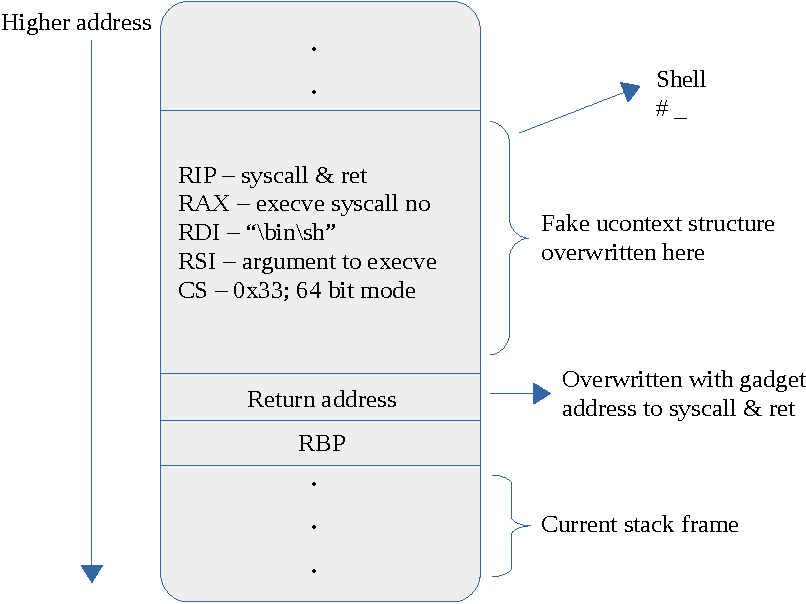
\includegraphics[height=2.5in, width=3in]{exploit}
\caption{Stack frame of exploit code}
\label{fig:SFEC}
\end{figure}

\section{Related Work}
For this work, \cite{bosman2014framing} is most relevant and a one 
stop reference. The paper provides detailed technical information 
on signal handling on UNIX based systems and introduces SROP as a 
generic exploitation technique. It also points to hints on abusing 
sigreturn system call, backdoor techniques based on SROP and ways to 
mitigate SROP attacks. 

\par In our current work, we have implemented a simple execve based 
exploit technique and a stack cookie based kernel level implementation
to address the exploitation as suggested in the paper. The paper authors
have also submitted a kernel patch targeting a different approach - counter
per process in the kernel space that keeps track of number of signal handlers
currently executing, the counter increases on signal delivery and decreases
on sigreturn path. Although this technique prevents SROP technique, it has
its own drawbacks in terms of counter roll-over and creates complications with
multi-threaded applications. We presume that these are some valid reasons why
the patch has not made it into the mainline kernel. In contrast, our approach 
is more elegant and leaves less to no room for the attacker to guess the cookie
value. Moreover, techniques suggested in the paper target older kernel versions, 
we have tested the exploit and the kernel fix on the latest kernel version (4.3).

\par As SROP is a type of an ROP attack, we find \cite{cowan1998stackguard}
related as this work implements a compiler feature which adds a cookie to the stack, 
as well as support to verify the cookie upon return of a function.  Buffer overflow 
attacks are probably the most famous form of attack gaining notoriety in the early 90's
The method works by modifying gcc such that it generates code that places a
32 bit identifier on the stack before the return address during a call instruction.
Also prior to a return gcc has the function call a verify method which validates 
that the 32 bit identifier is the same identifier that was placed there previously.
This research is very similar to the approach we have taken to prevent SROP.  
We utilize a stack cookie generated by the kernel to prevent an attacker from 
creating an arbitrary signal frame on the stack causing the kernel to jump arbitrarily 
through the code.

\par Another relevant reference is \cite{li2010defeating} as the work implements a 
compiler technique to prevent ret instructions from being generated in a kernel image. 
By removing ret instructions from the kernel it prevents an entire class of attack, 
Return Oriented Programming (ROP) from ever occurring because the fundamental feature 
of the attack is removed. The authors modify LLVM such that it will never generate a ret 
op-code, as well as will never generate a sequence of instructions that contain a ret op-code, 
if you were to jump between instructions. Instead of developing a technique to systematically 
remove the necessary elements for the attack we have used a hardening technique to 
prevent the attack.

% The following two commands are all you need in the
% initial runs of your .tex file to
% produce the bibliography for the citations in your paper.
\bibliographystyle{abbrv}
\bibliography{sigproc}  % sigproc.bib is the name of the Bibliography in this case
% You must have a proper ".bib" file
%  and remember to run:
% latex bibtex latex latex
% to resolve all references
%
% ACM needs 'a single self-contained file'!
%
% That's all folks!
\end{document}
